% % Permutation 1
% middle1(X, [X]).
% middle1(X, [First|Xs]) :-
%  append(Middle, [Last], Xs),
%  middle1(X, Middle).

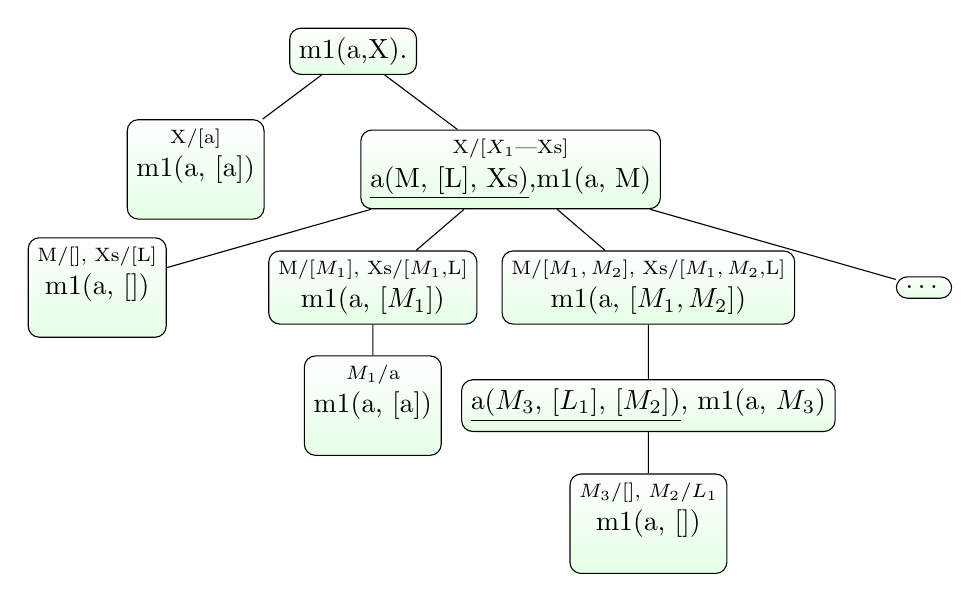
\begin{tikzpicture}[sibling distance=12em, align=center,
  every node/.style = {shape=rectangle, rounded corners,
    draw, align=center,
    top color=white, bottom color=green!10},
    level 1/.style={sibling distance=4cm},
    level 2/.style={sibling distance=3.5cm}, 
    level 3/.style={sibling distance=3cm}, ]
  \node {m1(a,X).}
    child { node {\scriptsize X/[a]\\m1(a, [a])\\$\blacksquare$}}
    child { node {\scriptsize X/[$X_1$|Xs]\\\underline{a(M, [L], Xs)},m1(a, M)}
      child { node {\scriptsize M/[], Xs/[L]\\m1(a, [])\\$\square$}}
      child { node {\scriptsize M/[$M_1$], Xs/[$M_1$,L]\\m1(a, [$M_1$])}
        child { node {\scriptsize $M_1$/a\\m1(a, [a])\\$\blacksquare$}}  
      }
      child { node {\scriptsize M/[$M_1,M_2$], Xs/[$M_1,M_2$,L]\\m1(a, [$M_1,M_2$])}
        child { node {\underline{a($M_3$, [$L_1$], $[M_2]$)}, m1(a, $M_3$)}
          child {node {\scriptsize $M_3$/[], $M_2/L_1$\\m1(a, [])\\$\square$}}
        }
      }
      child {node {\ldots}}
    };
\end{tikzpicture}